% Activate the following line by filling in the right side. If for example the name of the root file is Main.tex, write
% "...root = Main.tex" if the chapter file is in the same directory, and "...root = ../Main.tex" if the chapter is in a subdirectory.
 
%!TEX root =  ../Thesis.tex

\chapter[Reconstruction and Performance]{Event Reconstruction and Performance}
Once the physics data has been created by the LHC, detected by the ATLAS detector, and written to 
disk by the ATLAS trigger and data acquisition system, it is reconstructed into physics events.  This process has 
many interacting steps.  First, hits in the inner detector are algorithmically combined into tracks, which approximate the 
trajectory of charged particles, while energy clusters in the calorimeters are grouped together into jets, which seek to 
capture the energy of the particle that originated the jet.  

Higher-order quantities and corrections also come into play.  Two of the most important are the calibration and removal of 
pileup, other lower-energy interactions from the same or adjacent bunch crossings, and $b$-tagging
, which primarily uses tracks to identify jets that are likely originated by $b$-quarks.  Additionally, 
there are jet energy corrections that account for jet radiation that could by lost by the jet clustering algorithms, 
$b$-tagging efficiency corrections, and uncertainties on the total luminosity collected. 



\section{Track Reconstruction}
\label{sec:trk_reco}
%https://twiki.cern.ch/twiki/pub/AtlasPublic/EventDisplayStandAlone/2012_highPileup.png
Track reconstruction takes place in the inner detector and allows crucial measurements such as the primary and secondary vertices.  
When a charged particle traverses the layers of the inner detector, it leaves typically 8-11 hits in 
silicon (counting one double-sided layer of SCT silicon as capable of seeing 2 hits) and about 
35 in the TRT.  The track reconstruction algorithm, as detailed in section~\ref{sec:id_perf}, 
starts by identifying track seeds and then iterating through a Kalman filter algorithm, projecting out to further tracking layers 
and then checking for hits along the hypothesized trajectory of the particle.  

Track reconstruction performance can be impacted by pileup, as more pileup (and hence more tracking hits) creates 
more opportunities for incorrectly assigned hits and fake tracks from random hits being falsely associated with each other.  A 
second effect of pileup on tracking is indirect: the detector as a whole, and the silicon detectors in 
particular, undergo radiation damage as luminosity accrues.  Radiation damage in silicon detectors manifests 
itself as rising leakage current, which makes channels prone to more noise hits unless the thresholds are raised (
but higher thresholds lowers the efficiency for legitimate hits).  As time goes on, the tracking quality can can 
be affected by the extra noise hits and/or higher thresholds.

\begin{figure}
	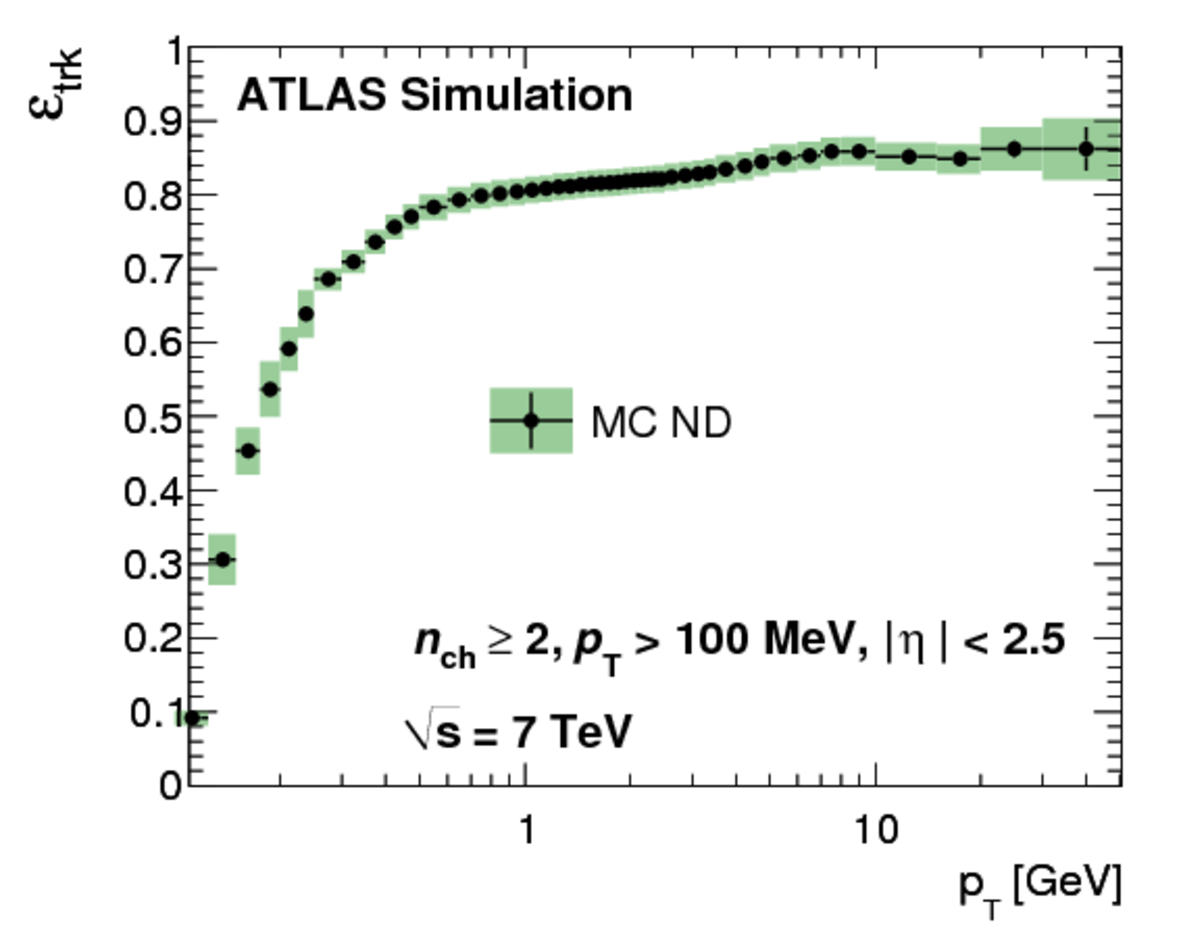
\includegraphics[width=0.5\textwidth]{ReconstructionPerformance/images/track_perf1.pdf}
	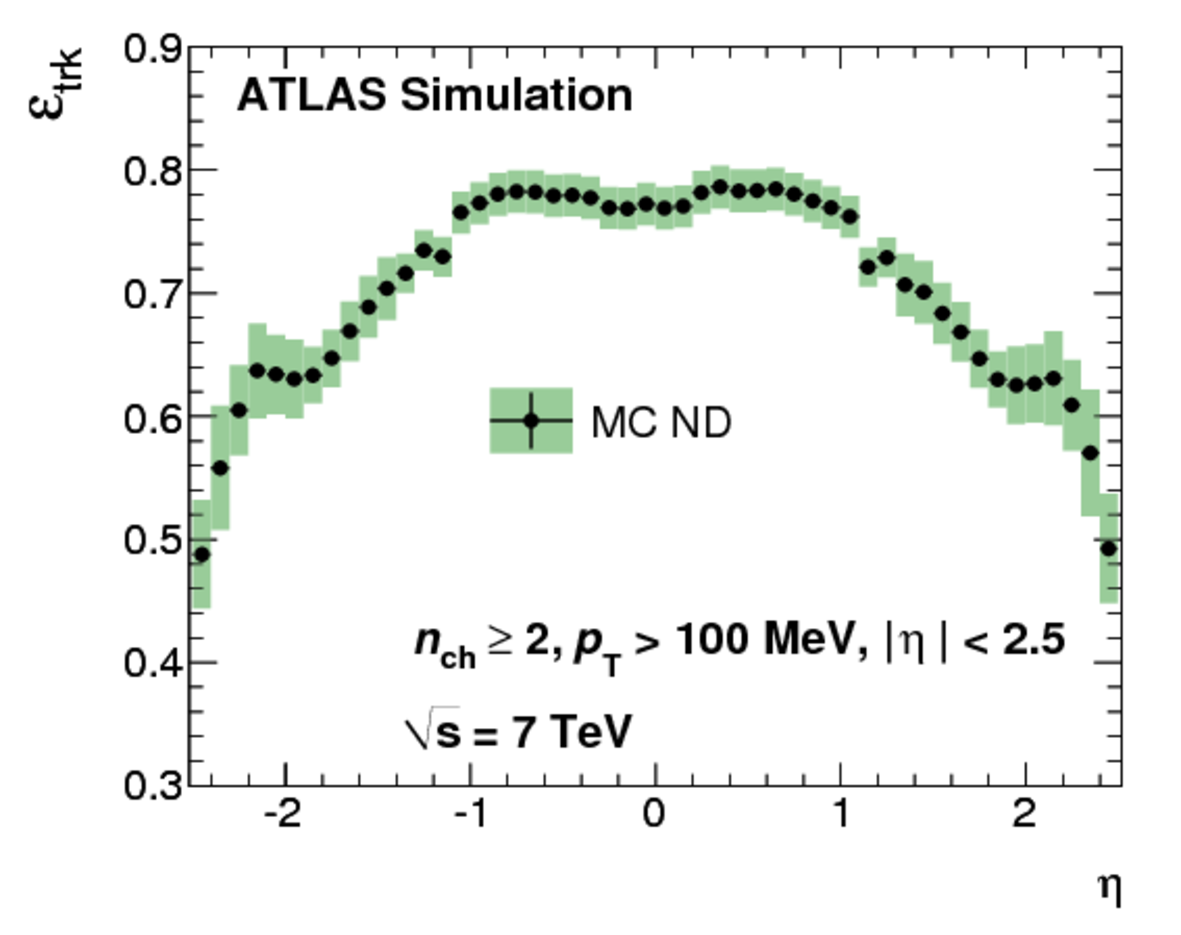
\includegraphics[width=0.5\textwidth]{ReconstructionPerformance/images/track_perf2.pdf}
	\label{fig:track_perfA}  
	\caption{The efficiency of the track reconstruction, projected in $p_T$ and $\eta$, as computed in Monte Carlo.}
\end{figure}



\begin{figure}
	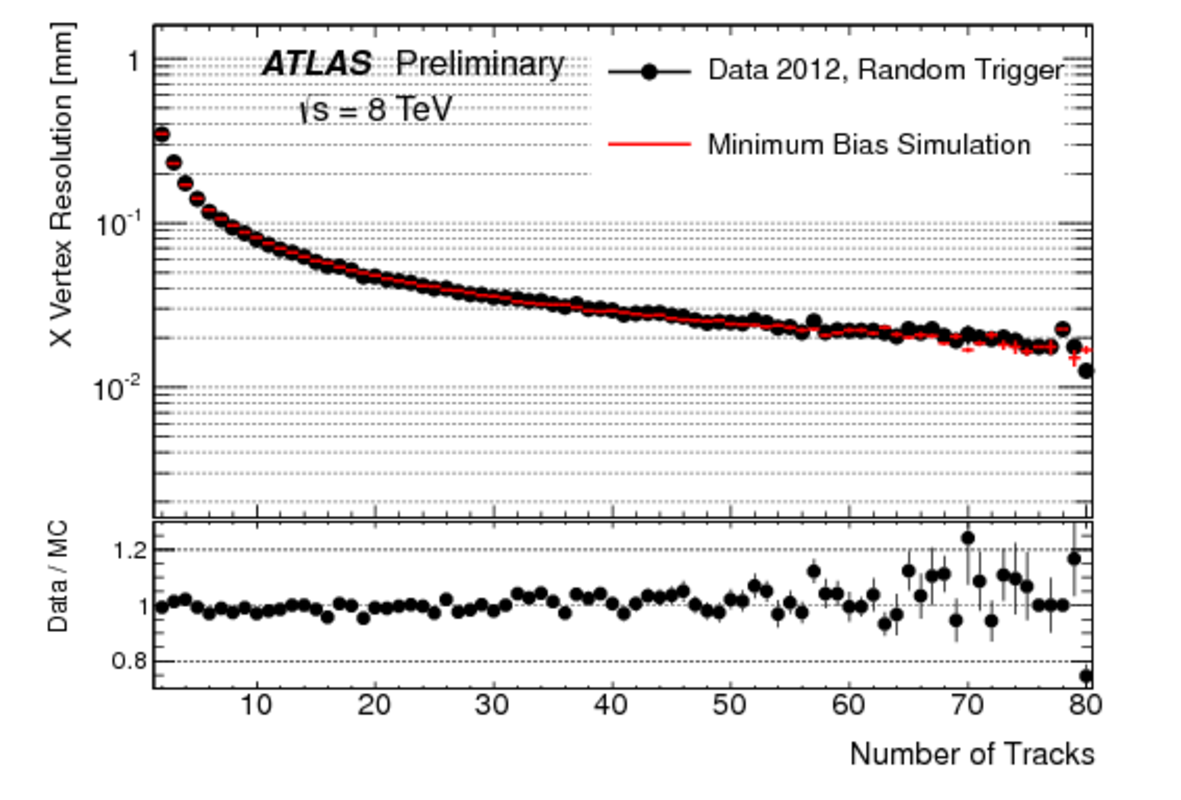
\includegraphics[width=0.5\textwidth]{ReconstructionPerformance/images/track_perf3.pdf}
	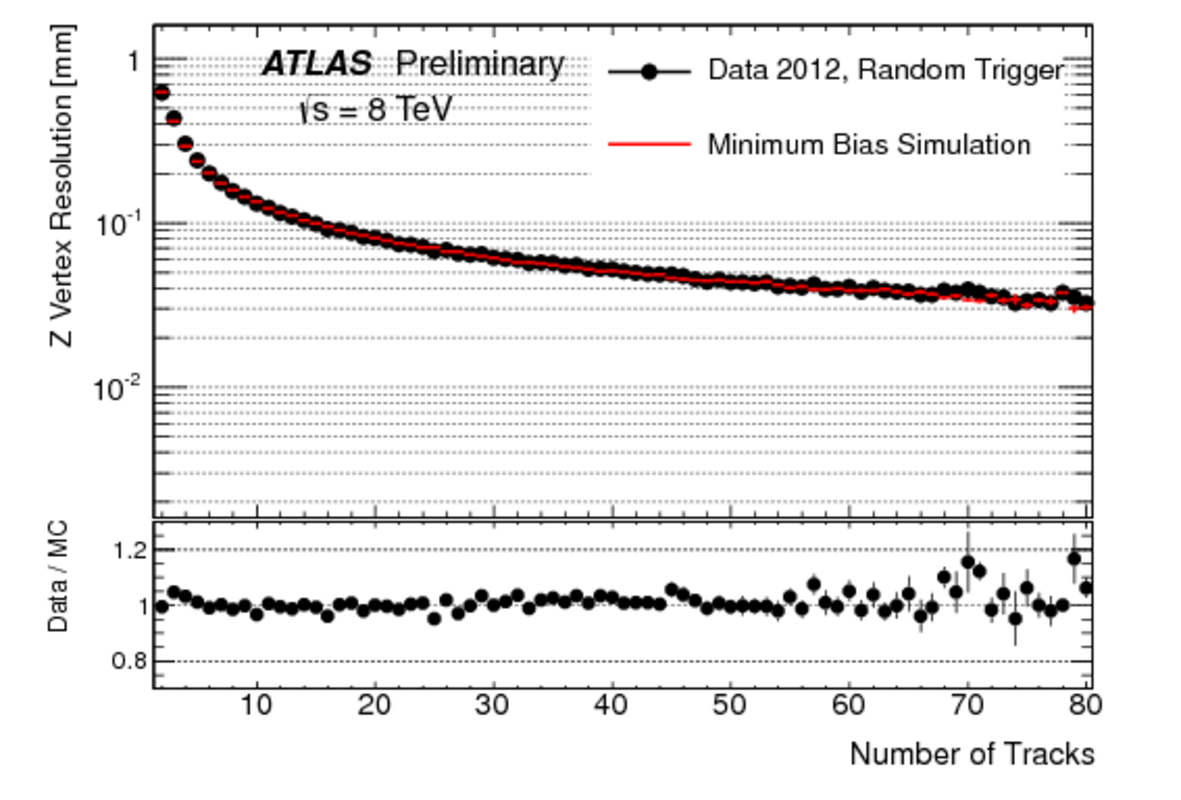
\includegraphics[width=0.5\textwidth]{ReconstructionPerformance/images/track_perf4.pdf}
	\label{fig:track_perfB}  
	\caption{The track resolution in mm the $x$ and $z$ directions, comparing minimum bias simulation to data taken with a random trigger.}
\end{figure}

Good tracking performance enters this analysis most directly in its impact on the tagging of $b$-jets, as detailed in Section~\ref{sec:b-tag}.  Well-reconstructed tracks allow for the identification of a secondary vertex, which is one of the fundamental features of the ATLAS $b$-jet tagging algorithms.

% http://www.slac.stanford.edu/cgi-wrap/getdoc/slac-pub-5671.pdf
% http://www.quantumdiaries.org/2011/06/10/to-b-or-not-to-bbar-b-tagging-via-track-counting/
% http://dorigo.wordpress.com/2007/05/15/b-hadron-lifetimes-part-2/

% http://iopscience.iop.org/1742-6596/119/3/032014/pdf/1742-6596_119_3_032014.pdf
\subsubsection{Inner Detector Performance and Tracking}
\label{sec:id_perf}
Measurements from the pixel, SCT and TRT are combined in the track reconstruction.  There is a broad range 
of properties that tracks might have, so the inner detector has to be able to measure tracks with p$_T$
 ranging from 150 MeV to 30 GeV or more.   

The main track reconstruction algorithm used at ATLAS is a version of the Kalman filter algorithm.  The track reconstruction 
begins with track seeds, which are collections of a few hits in the pixel subsystem that could plausibly be 
parts of tracks.  The advantage of starting with seeds, rather than attempting to find an entire track at 
once, is that seeds allow flexibility at the beginning of the search (when the track trajectory is the 
least known) while keeping computational costs down.  Once a seed has been identified, the Kalman fitter (
as the ATLAS algorithm is called) projects where the next hit would be if there is truly a track 
present, and then looks for the presence of a hit at the predicted location in the next tracker layer
.  If a hit is found there, the predicted trajectory of the particle may be refined and the next 
hit is predicted and sought, until all the detector layers have been traversed. If there is no hit 
present where one is predicted, the Kalman fitter can project two layers further, to allow for the possibility 
of a hole where the particle did not leave a hit for some reason. 

In high-pileup environments, the inner detector occupancy can be high which can make for two tracks that 
overlap, leaving a hit in the same place which must then be allocated to one or the other.  
Dedicated ambiguity solving is implemented as a second stage in the track reconstruction, where the two candidate tracks are 
scored against each other via a reward/penalty scheme.  A good $\chi^2/DOF$ 
score is rewarded, a track with many holes on track or a low $\chi^2/DOF$ 
is penalized, with subdetector-specific weighting favoring the higher-precision silicon over the the lower-precision TRT. 



%http://arxiv.org/pdf/0802.1189.pdf
%http://iopscience.iop.org/1126-6708/2008/04/063/pdf/1126-6708_2008_04_063.pdf
\section{Jet Reconstruction}
\label{sec:jet_reco}
Because of asymptotic freedom of QCD, quarks and gluons do not remain standalone particles once they're produced
, but instead they hadronize and shower as they travel through the detector.  Hypothetically, all the particles of 
the shower can be added back up to approximate the energy, momentum, and angle of the original quark 
or gluon.  Jet reconstruction is the process of assembling calorimeter deposits together into a physics object, called a 
jet, that ideally will do a good job of representing the characteristics ($p_T$, energy, 
flavor) of the quark or gluon that originated the jet.  There are a number of clustering algorithms for 
assembling the calorimeter cells, and post-processing steps for improving the performance of jets in analyses--pileup 
subtraction, energy calibrations, grooming, and trimming, to name a few.  

The default jet clustering algorithm in ATLAS is the anti-$k_t$ algorithm \cite{antikt}
with a distance parameter of 0.4.  Roughly summarized, this algorithm starts with a calorimeter cell that 
has an energy deposit at least $4\sigma$ higher in energy than the ambient and pileup noise, 
and then the surrounding cells with at least $2\sigma$ more energy than noise are grouped into 
the jet in a way that prioritizes high energy over close proximity.  The result is that soft deposits get 
clustered in with hard deposits, rather than clustering amongst themselves.  The distance parameter of 0.4 is 
a cutoff as to how far away from the seed in $\eta-\phi$ space to look for 
additional deposits.   Jets below 20 GeV or so can be difficult to distinguish from noise, so in practice, a lower limit on 
the $p_T$ (in the case of this analysis, 25 GeV) is often applied.  

A critical feature of this algorithm, or any jet algorithm, is that it be infrared and collinear safe
.  In technical terms, that means that when additional `ghost' particles with infinitesimally small energy or infinitesimally 
close radius are added to the area in and around the jet, the properties of the resulting jet do 
not change.  In practical terms, it means that the jet is stable to small perturbations, so that 
the presence or absence of low-energy nearby radiation (which can be difficult or impossible to distinguish from 
calorimeter noise) or the precise direction of energy that is highly collinear with the jet itself (the direction 
of this energy can be prone to resolution uncertainties) do not affect the jet properties.  Critically, the 
anti-$k_t$ algorithm is both infrared and collinear safe.







%https://twiki.cern.ch/twiki/bin/view/AtlasPublic/LuminosityPublicResults#Data_Taking_Efficiency_and_Pileu

\section{Pileup Calibration and Removal}
\label{sec:pileup}
All the detector subsystems are affected by the presence of pileup, which are collisions other than the hard scatter 
collision.  As the LHC delivers higher luminosity for a given number of proton bunches, the luminosity increase comes 
at the price of many interactions per bunch crossing, and these softer interactions create extra activity in the detector 
that tends to make events noisier and more challenging to reconstruct accurately.  In 2012, the mean number of 
interactions per crossing ranged from about 10 up to about 40.  

The inner detector and tracking provide an important tool for understanding in-time pileup.  In-time pileup 
is additional soft interactions in the same bunch crossing as the hard scatter.  The tracking allows primary vertex reconstruction 
with a resolution fine enough in z$_0$, for the pixels typically $z_0\sin\theta$, 
to resolve separate primary vertices from each other \cite{pileup_tracks}.   The calorimeters cannot resolve individual primary vertices with such precision, 
though, so a constant struggle in ATLAS is to measure the calorimeter deposits that come from pileup interactions, 
and where possible to apply corrections that subtract away pileup contributions to jets from the hard scatter.  On average
, each additional pileup vertex in an event adds 370(850) \cite{pileup} MeV to the p$_T$ of a jet reconstructed with the Anti-kT algorithm with R=0.4(0.6).

In addition to in-time pileup, the calorimeters are prone to out-of-time pileup where 
the signal in a given in event can be affected by the energy flow of previous collisions because of the 
calorimeter readout signal shapes.  Out-of-time pileup has the effect of adding an average of 60
(210) MeV to central jets, and decreasing the forward jets by 350(470) MeV.  


\begin{figure}
	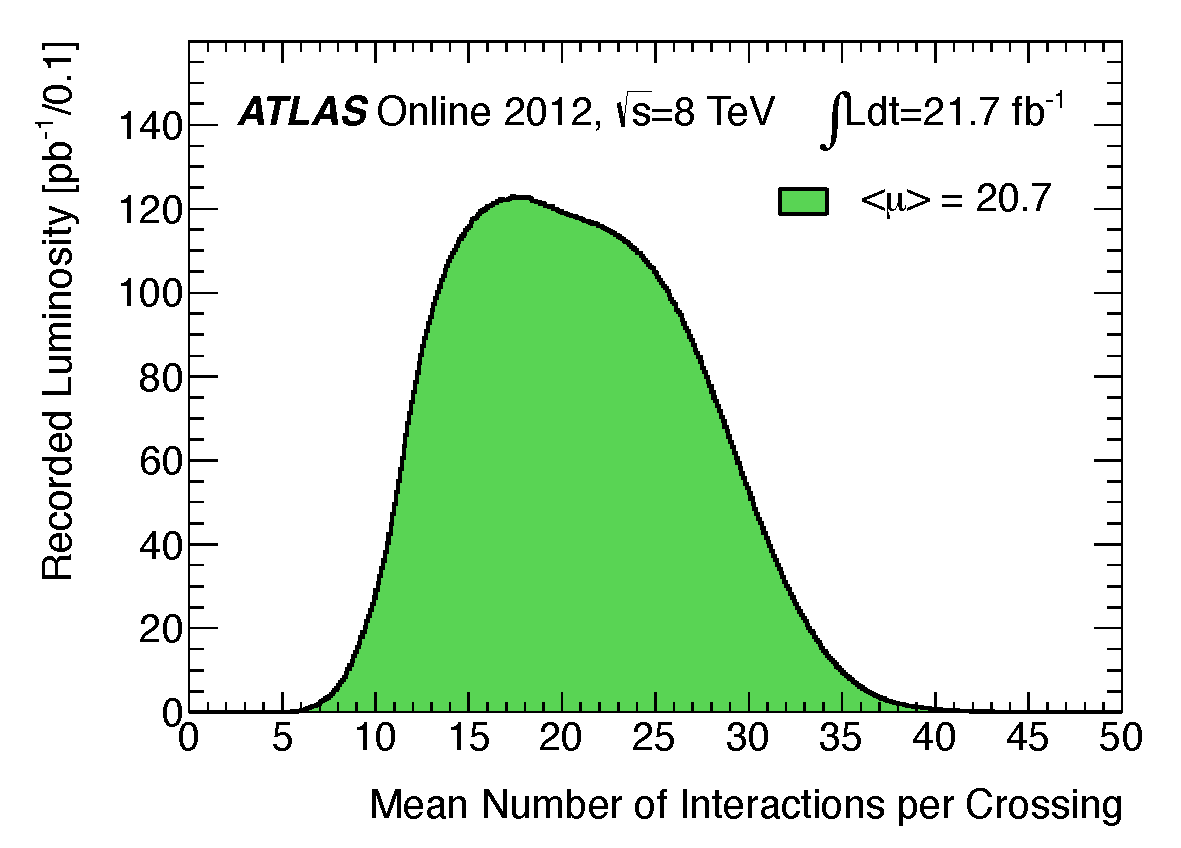
\includegraphics[width=0.8\textwidth]{ReconstructionPerformance/images/mu_2012-dec.pdf}
	\caption{A distribution of the mean number of interactions per crossing, also called $\mu$ seen in 2012 data-taking.  Larger $\mu$ values are characterized by more challenging reconstruction. 	\label{fig:mu_2012}  }
\end{figure}

% http://cds.cern.ch/record/1435196/files/ATLAS-CONF-2012-042.pdf
%http://iopscience.iop.org/1742-6596/119/3/032033/pdf/1742-6596_119_3_032033.pdf
\section{Primary Vertex Identification}
\label{sec:pv}
Both the hard scatter collision and pileup collisions produce charged tracks; once these tracks are reconstructed, they can 
be traced back to the interaction region of the ATLAS detector and used to figure out where collisions took place
.  Each time a group of tracks can be clustered together into a presumed collision, we refer to it 
as a primary vertex.  The reconstruction of primary vertices is one of the reasons that tracking resolution must be 
so precise; primary vertices are often separated by only a few mm so imprecisely measured tracks can cause unintended 
merging.  The consequence of mistakes in the primary vertex reconstruction can be physics objects that get grouped with the 
wrong primary vertex, and lead to incorrect event reconstruction and either signal loss or undesired background acceptance.

The reconstruction errors on the primary vertex are generally within 0.02 mm in the x/y directions 
(transverse to the beam direction) and 0.1 mm in the z direction (longitudinal to the  
beam) \cite{pileup_tracks}.   This resolution can be seen in Figure~\ref{fig:pileup_pv}, a 2012 
$Z\rightarrow\mu\mu$ event with 25 reconstructed primary vertices.



%-----------------------------------------------------------------------------
\begin{figure}
	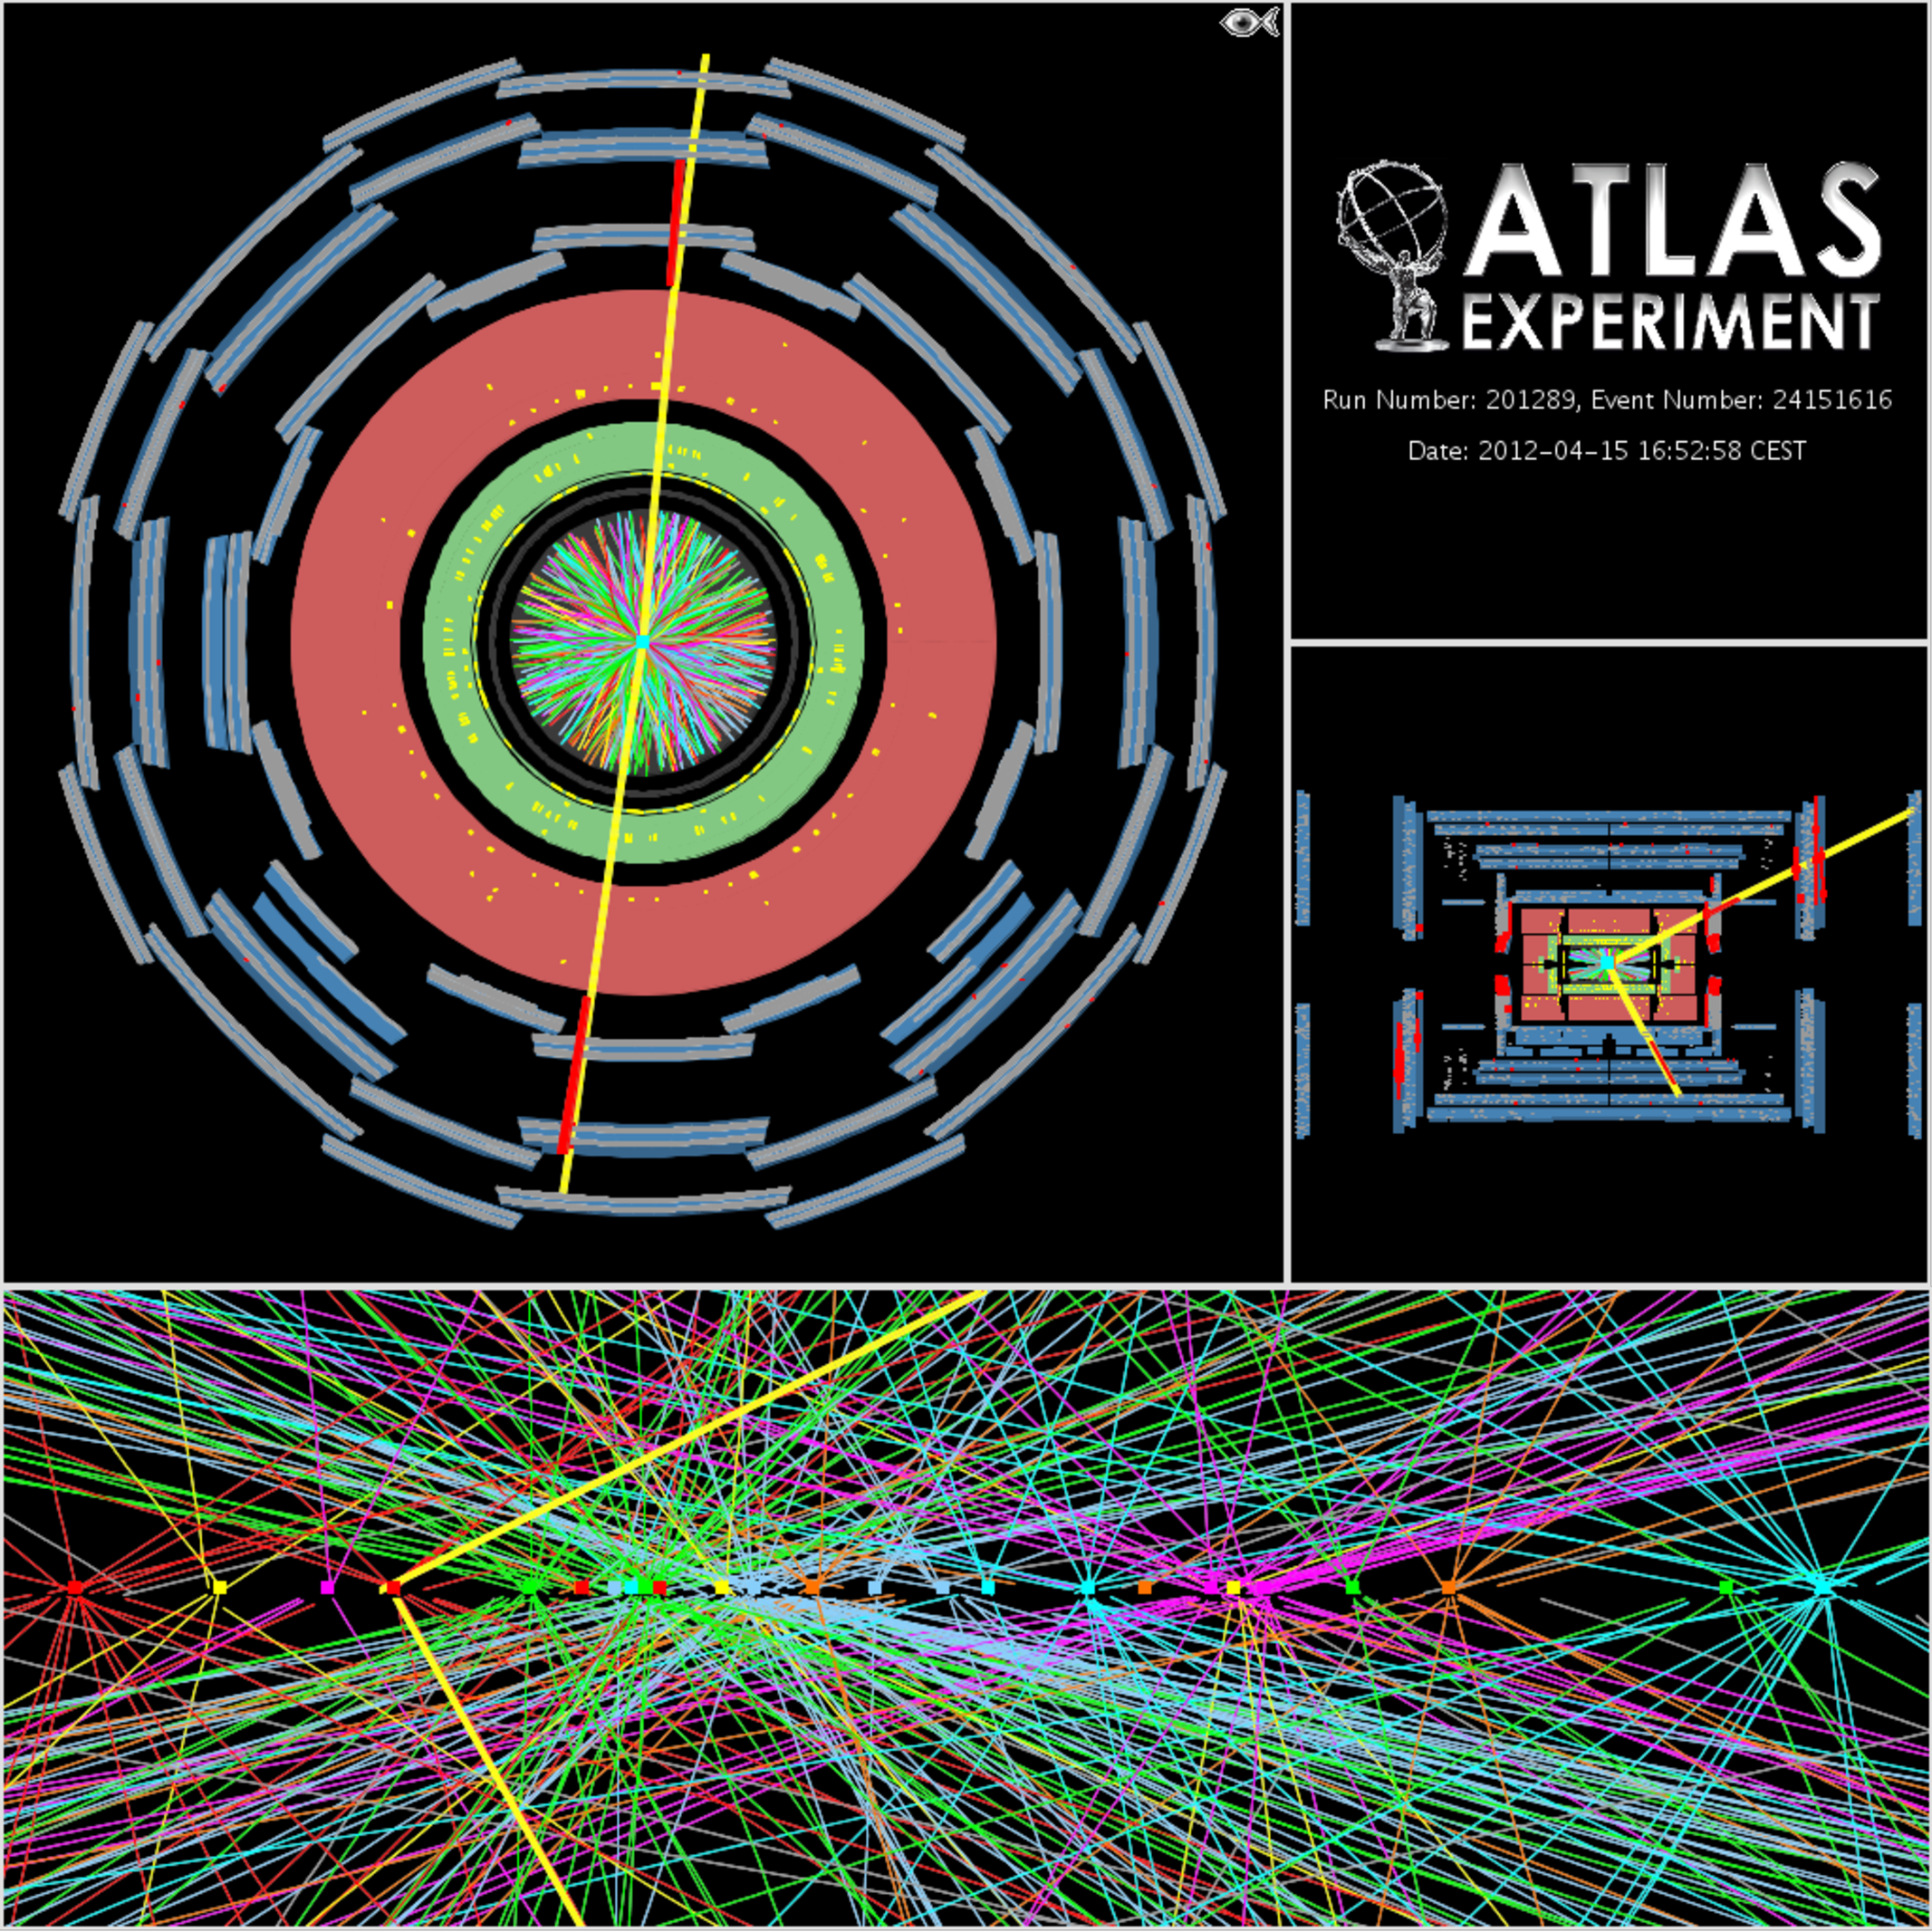
\includegraphics[width=0.8\textwidth]{ReconstructionPerformance/images/2012_highPileup.pdf}
	\caption{A data event taken in 2012, showing the occupancy typical of high pileup. 	\label{fig:pileup_pv}  }
\end{figure}
%-----------------------------------------------------------------------------


\section{$b$-Tagging}
\label{sec:b-tag}
B quarks typically have a lifetime of about 1ps
, and since they are often created in high-p$_T$ collisions or come from the decay 
of heavy particles, they can have considerable $p_T$ and travel a few millimeters before decaying
.  B-tagging algorithms typically look for evidence of secondary decay vertices that are displaced from the beamspot in 
the transverse direction.   



Another critical tool built on top of good tracking is $b$-tagging, or identifying jets that likely 
came from $b$-quarks.  A unique feature of $b$-quarks relative to other strongly interacting 
particles is the long lifetime of $b$-quarks, which means that they can travel a few mm 
out from the primary vertex before decaying.  This feature of $b$-jets means they can be identified 
by the presence of one or more kinematic characteristics:


%-----------------------------------------------------------------------------
\begin{itemize}
	\item large significance of the impact parameter, $d_0$ (IP3D)
	\item large ratio between the sum of $p_T$ of all tracks associated with the secondary vertex to the sum of all tracks in the jet (SV1)
	\item large secondary vertex mass (SV1)
	\item evidence of a decay chain including both a secondary vertex (from the $b$ decay) and a tertiary vertex (from the $c$ quark daughter of the $b$ quark) along the same line of flight (JetFitter)
\end{itemize}

\begin{figure}
	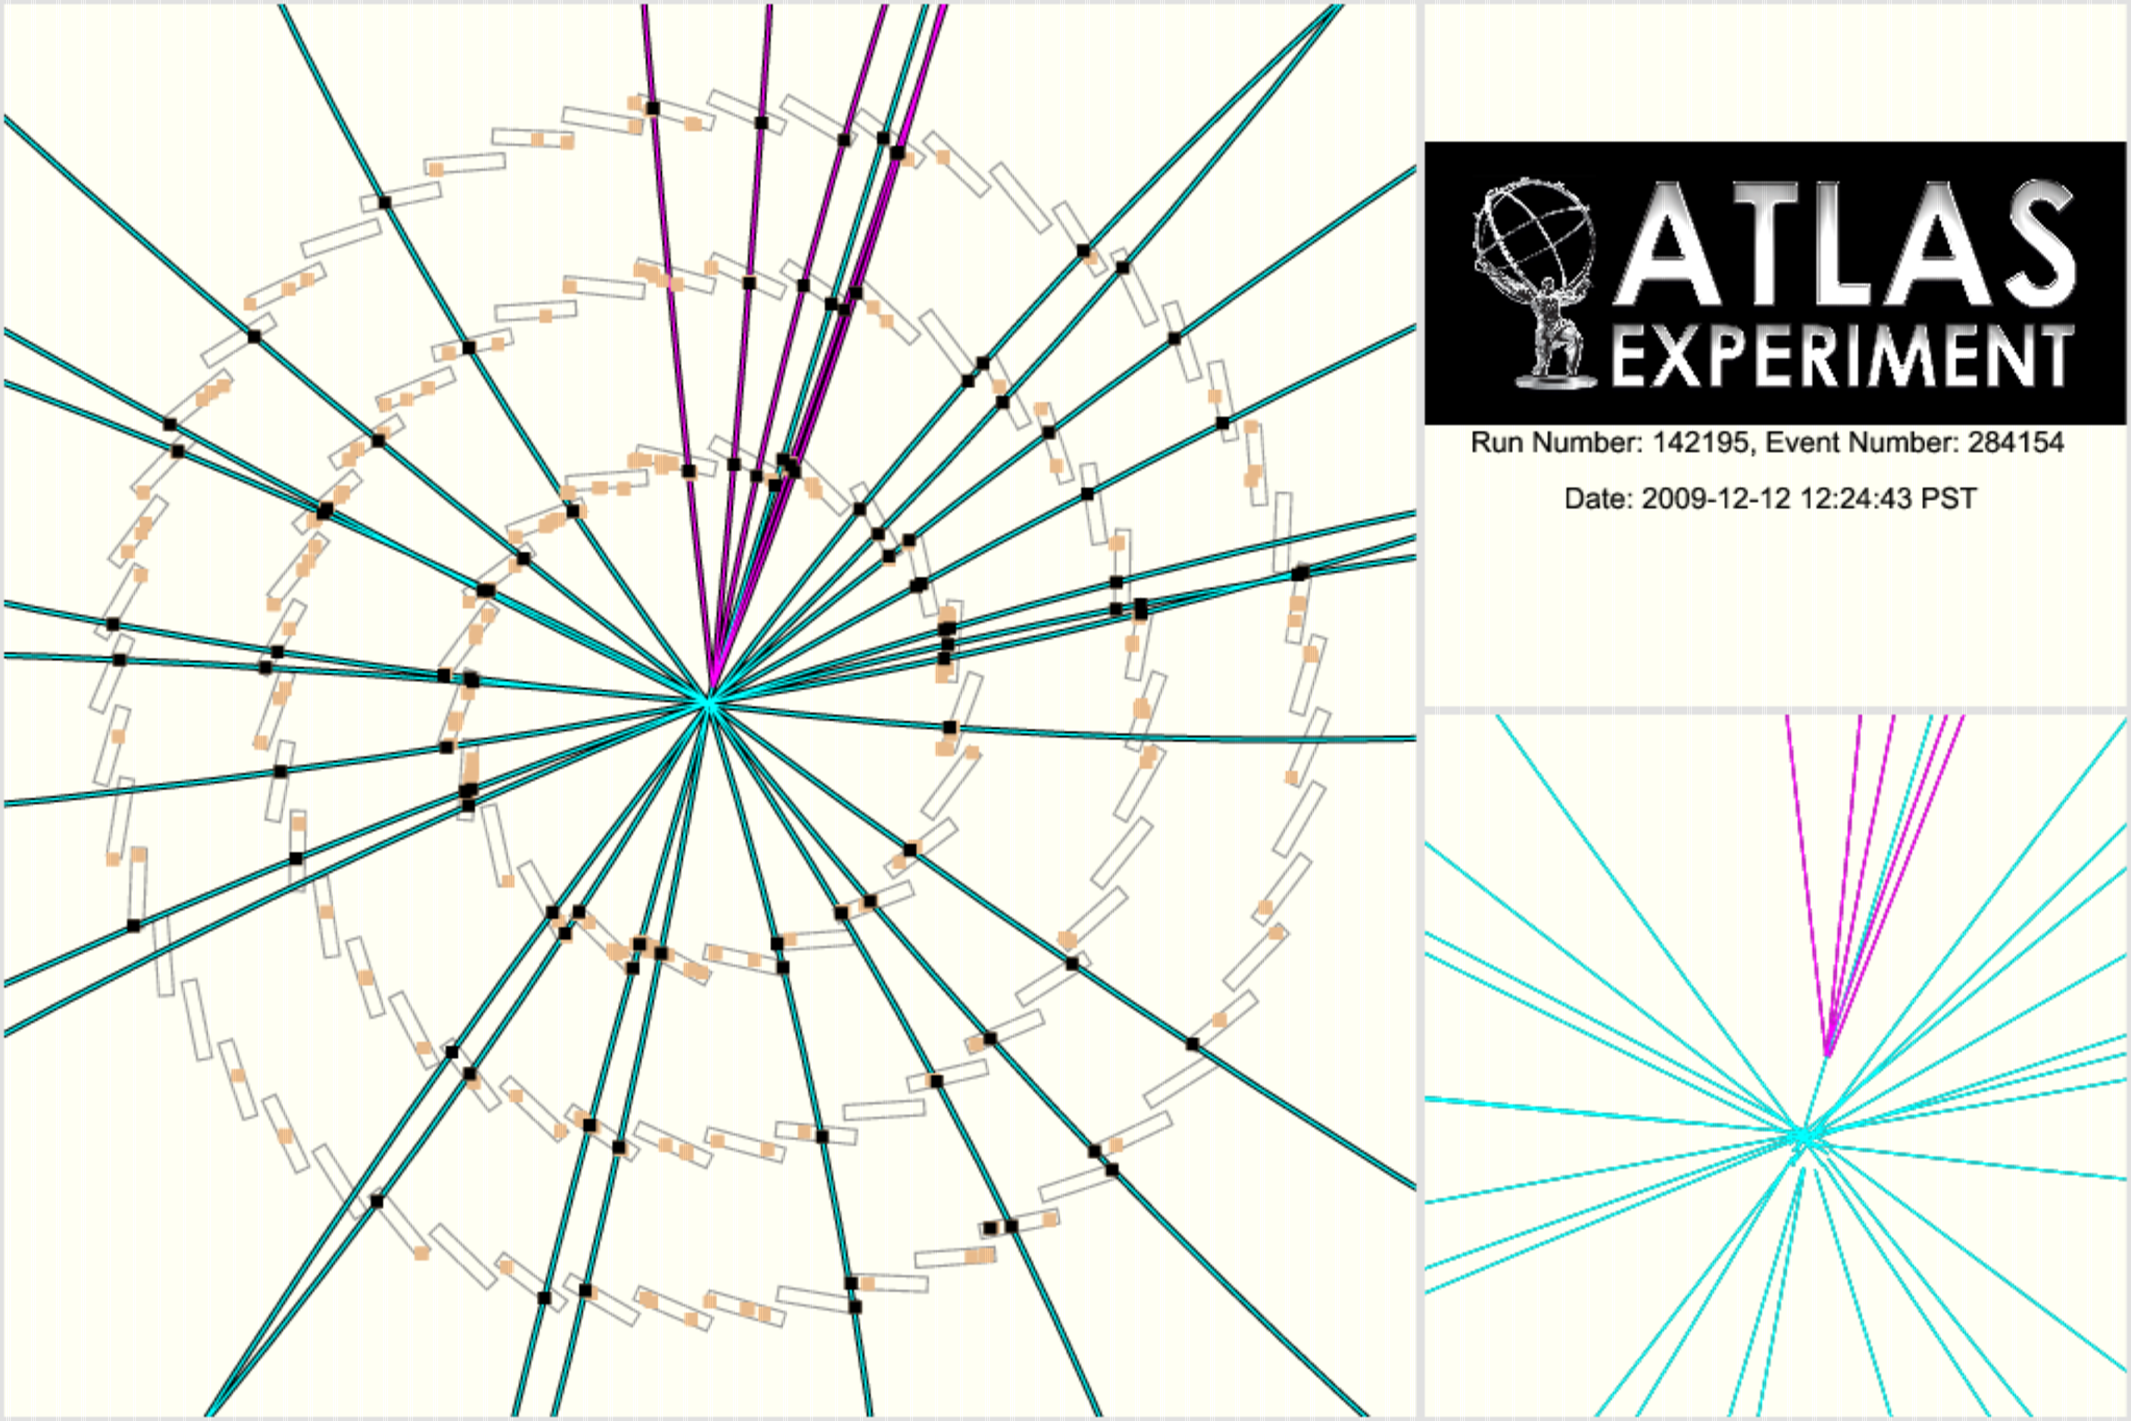
\includegraphics[width=0.8\textwidth]{ReconstructionPerformance/images/secondary_vertex.pdf}
	\caption{An event from early ATLAS data-taking, with a number of tracks (in teal) leading back to the primary vertex, and a secondary vertex reconstructed with the associated tracks highlighted in purple \cite{sv}.	\label{fig:secondary_vertex}  }
\end{figure}
%-----------------------------------------------------------------------------




There are several different $b$-tagging algorithms that exploit each of these features independently; however, if 
a jet truly comes from a $b$-quark, then several of these features can arise in the 
same jet and the correlation can be used to further increase the accuracy of the tagger.  That idea gives 
rise to the MV1 tagger (where the MV stands for ``multivariate''), a neural-net-based 
$b$-tagging algorithm that uses three other $b$-tagging algorithms (SV1, IP3D, JetFitter
) as inputs.   The performance curve for the MV1 algorithm can be seen in Figure~\ref{fig:mv1_roc}; 
for a typical $b$-jet efficiency of 70\% (meaning that 70\% of real $b$-jets 
are positively tagged by the algorithm), the light-jet rejection is about 99.5\% and the 
charm rejection is about 90\% \cite{b-tagging}.


%https://atlas.web.cern.ch/Atlas/GROUPS/PHYSICS/CONFNOTES/ATLAS-CONF-2014-046/fig_01.pdf
\begin{figure}
	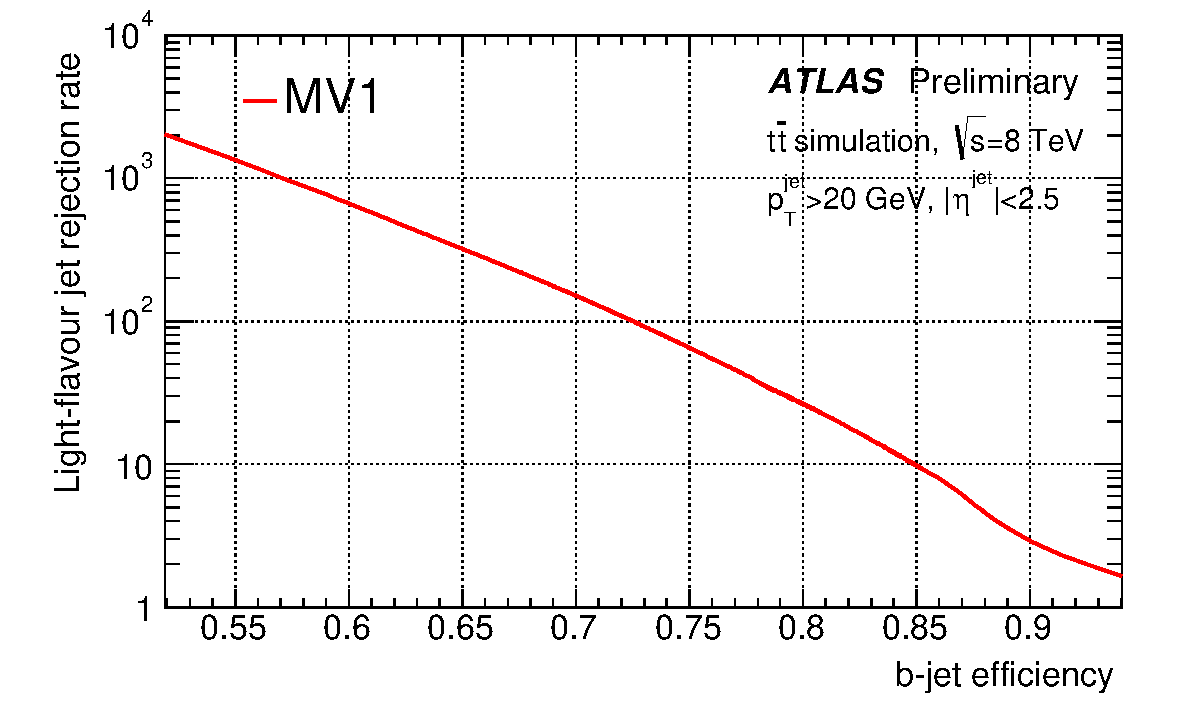
\includegraphics[width=0.8\textwidth]{ReconstructionPerformance/images/mv1_roc.pdf}
	\caption{secondary vertex \cite{b-tagging}	\label{fig:mv1_roc}  }
\end{figure}
















